\section{Die Bibel}
\subsection{Grundlegendes}
\subsubsection{Was ist die Bibel?}
Die Bibel ist das meist verkaufte Buch auf dieser Welt. Mit rund 35 Millionen Bibeln \folie{2} wurden 2022 weltweit vertrieben. Ob es auch das meist gelesene ist? Das Buch hat in der deutschen Übersetzung rund 1200--1400 Seiten \folie{3}. Also ein ordentlicher Schinken dieses Buch. Aktuell wurde dieses Buch in ca. 3600 Sprachen übersetzt. Das vollständige Buch, also das Neue und das Alte Testament in 743 Sprachen.\folie{4} 

Ursprünglich wurde das alte Testament in Hebräisch und kleine Teile in aramäisch geschrieben. Das neue Testament wurde in griechisch geschrieben. Später wurde von der Kirche ins lateinische übersetzt. Viel Jahrhunderte gab es die Bibel hier in Europa nur auf lateinisch. Martin Luther hat, dann die ganze Bibel ins Deutsche übersetzt. Er versuchte bei der Übersetzung das umgangssprachliche Deutsch in der damaligen Zeit einfließen zu lassen. Ein paar Jahre vorher wurde die Druckerpresse erfunden 
\begin{figure}
    \centering
    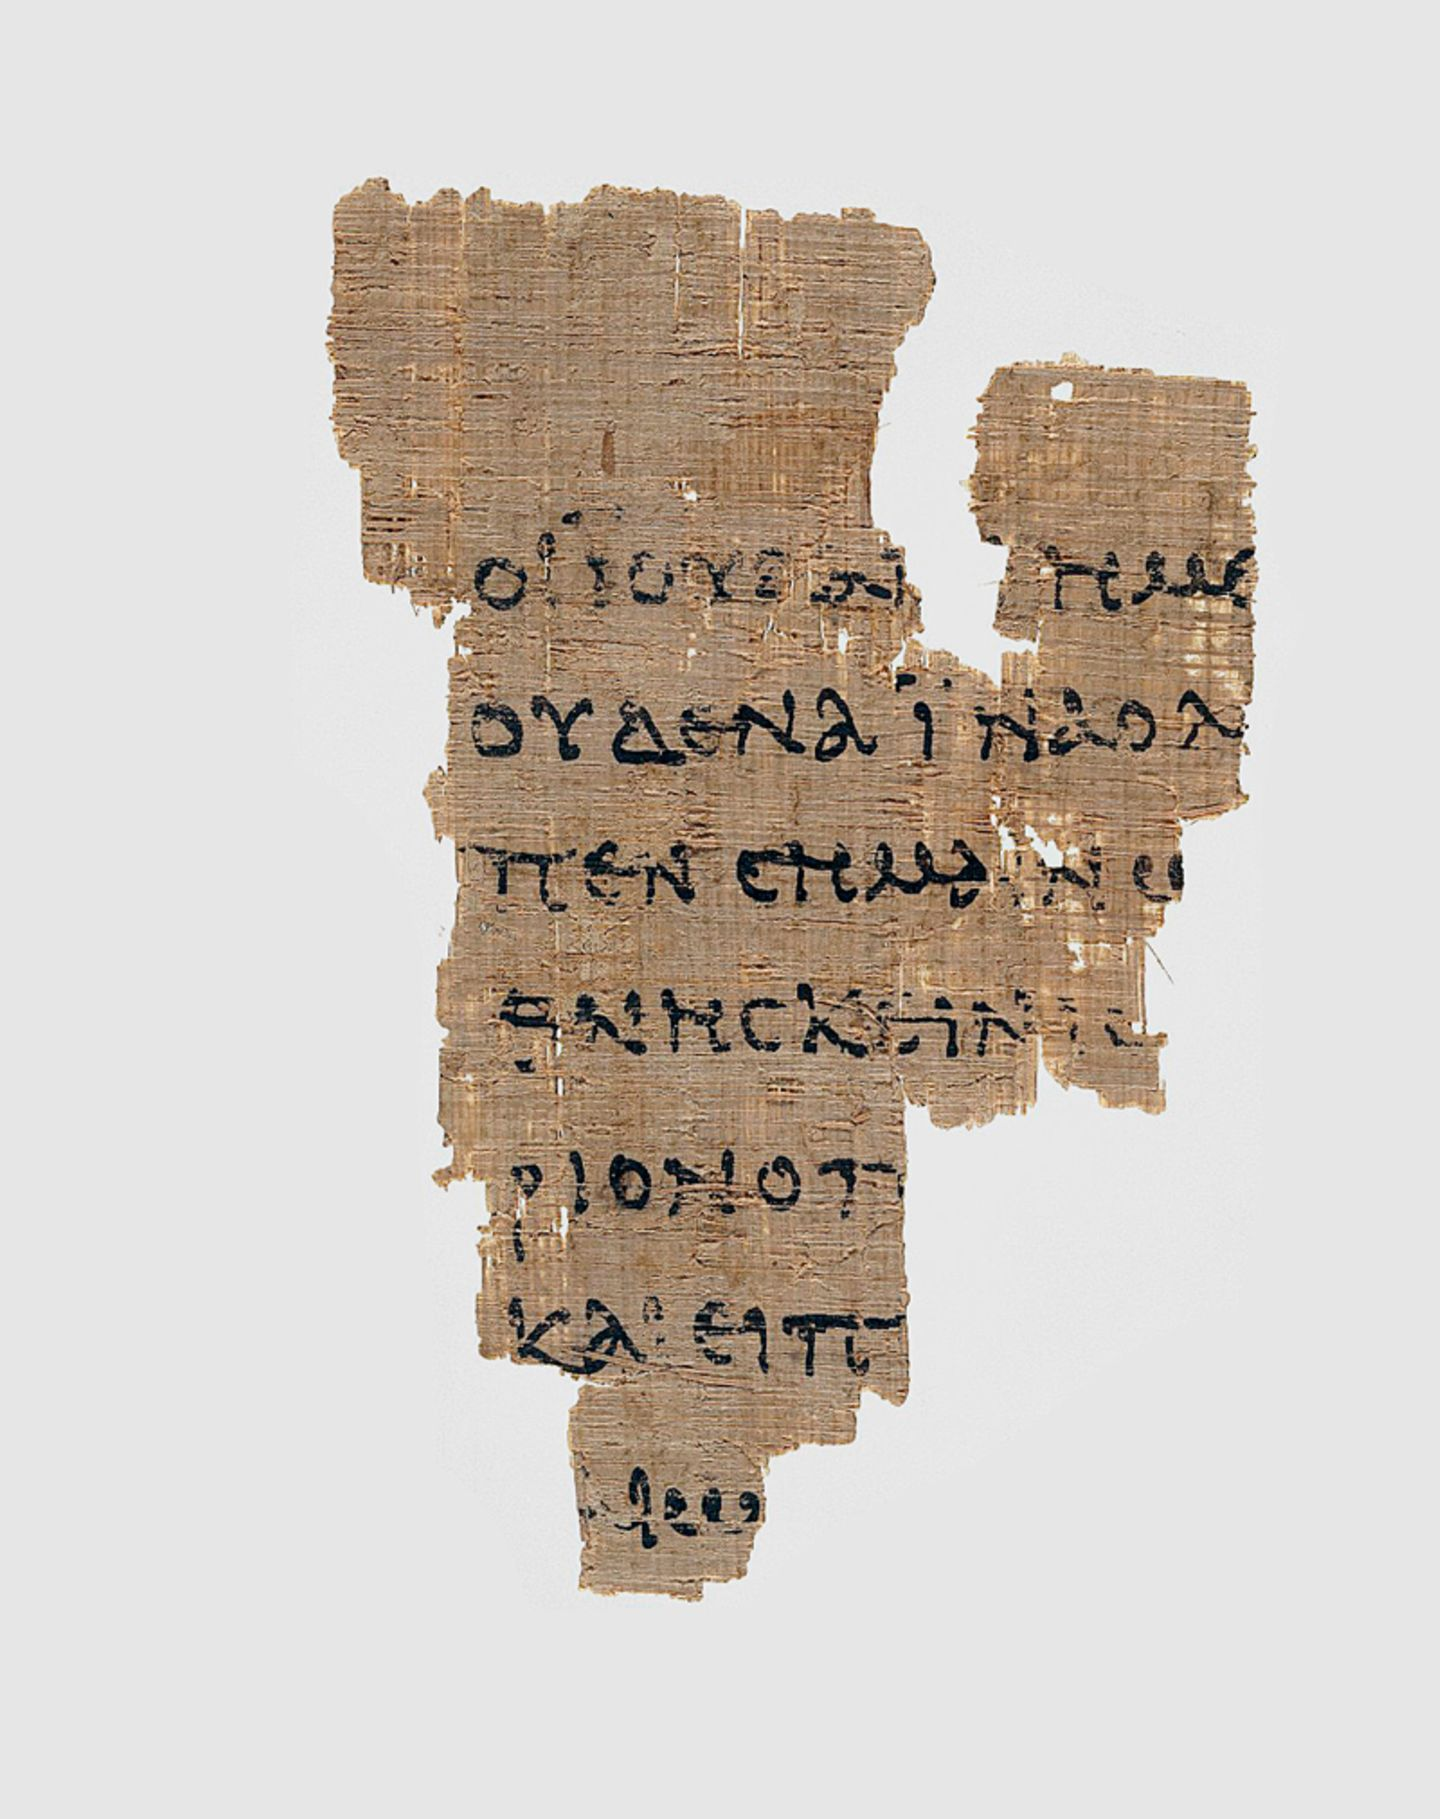
\includegraphics[width=0.5\linewidth]{src/Vorträge/BibelBuch/images/papyrusFragment.jpg}
    \caption{Dieses Papyrusfragment von etwa 125 n. Chr. ist der älteste Beleg für das Neue Testament. Er handelt vom Prozess gegen Jesus: Die Frage »Bist du der König der Juden?« ist teilweise zu entziffern\\
©John Rylands Library}
    \label{fig:enter-label}
\end{figure}